\documentclass[11pt,aspectratio=169]{beamer}

\usepackage{rcstalk}
\usetheme{rcstheme}

\topic{I/O and disks}
\subtitle{Lecture 11: I/O and Disks}

\begin{document}

\maketitle

\section{Computer Bus and Device Architecture}

\begin{slide}{Memory and I/O buses}
\begin{centering}
\input{bus.tex}\\
\end{centering}
\itms{
  \item CPU accesses physical memory over a bus
  \item Devices access memory over I/O bus with DMA
  \item Devices can appear to be a region of memory
}
\end{slide}

\begin{slide}{Realistic PC architecture}
\centerline{\input{bridge.tex}}
\end{slide}


\begin{slide}{What is memory?}
\itms{
  \item SRAM -- Static RAM
  \ittms{
    \item Like two NOT gates circularly wired input-to-output
    \item 4--6 transistors per bit, actively holds its value
    \item Very fast, used to cache slower memory
  }
  \item DRAM -- Dynamic RAM
  \ittms{
    \item A capacitor + gate, holds charge to indicate bit value
    \item 1 transistor per bit -- extremely dense storage
    \item Charge leaks---need slow comparator to decide if bit 1 or 0
    \item Must re-write charge after reading, and periodically refresh
  }
  \item VRAM -- ``Video RAM''
  \ittms{
    \item Dual ported, can write while someone else reads
  }
}
\end{slide}

\begin{slide}{What is I/O bus?  E.g., PCI}
\centerline{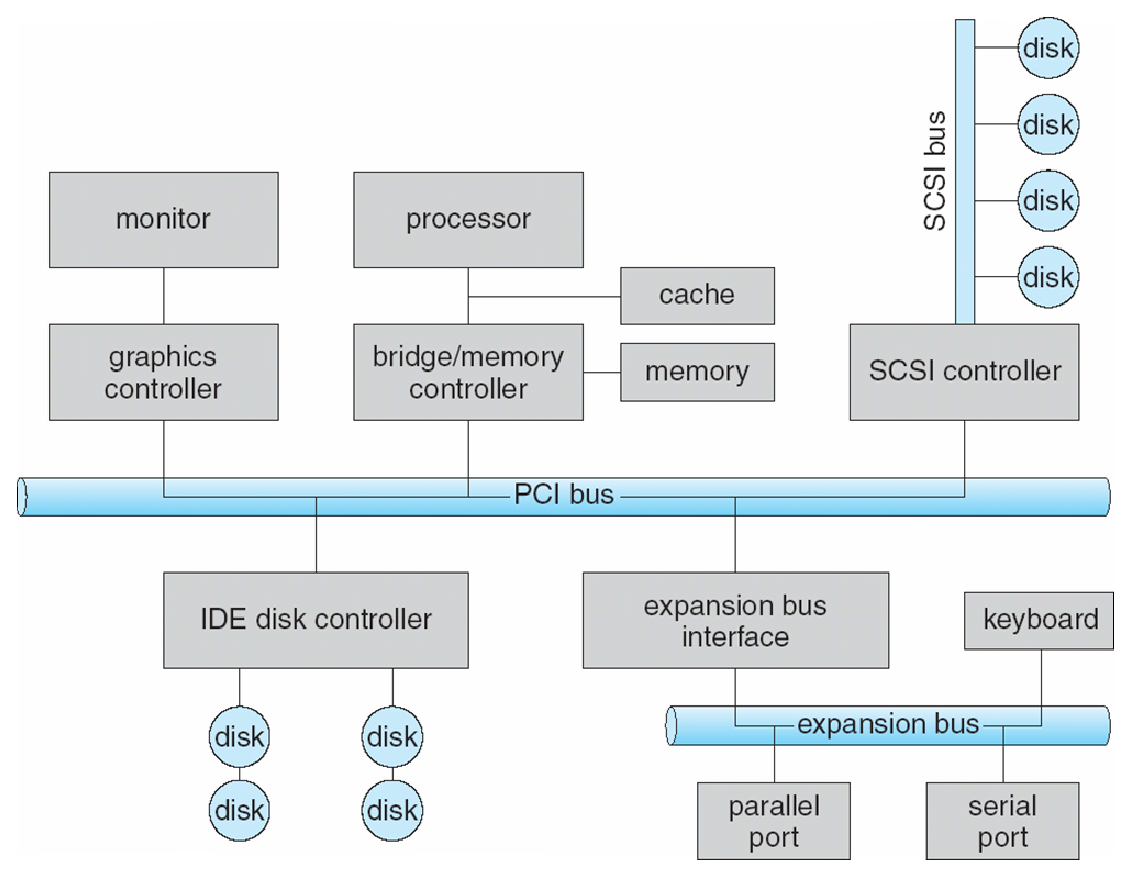
\includegraphics[height=2.8in]{figs/pci}}
\end{slide}

\section{Device Drivers}

\begin{slide}{Communicating with a device}
\itms{
  \item Memory-mapped device registers
  \ittms{
    \item Certain \emph{physical} addresses correspond to device registers
    \item Load/store gets status/sends instructions -- not real memory
  }
  \item Device memory -- device may have memory OS can write to
	  directly on other side of I/O bus
  \item Special I/O instructions
  \ittms{
    \item Some CPUs (e.g., x86) have special I/O instructions
    \item Like load \& store, but asserts special I/O pin on CPU
    \item OS can allow user-mode access to I/O ports with finer
	  granularity than page
  }
  \item DMA -- place instructions to card in main memory
  \ittms{
    \item Typically then need to ``poke'' card by writing to register
    \item Overlaps unrelated computation with moving data over
  (typically slower than memory) I/O bus
  }
}
\end{slide}

\begin{frame}
\frametitle{Example: parallel port (LPT1)}
\begin{itemize}
  \item Simple hardware has three control registers:\\[1ex]
{\hspace*{1em}\scriptsize
  \begin{tabular}{@{\vrule width0pt height 1.2em}|c|c|c|c|c|c|c|c|}
\hline
$D_7$&$D_6$&$D_5$&$D_4$&$D_3$&$D_2$&$D_1$&$D_0$\cr
\hline
\multicolumn{8}{c}{\sf read/write data register (port
    0x378)}\\[1.5ex]
\hline
$\overline{\mbox{BSY}}$&$\overline{\mbox{ACK}}$&PAP& \omit\hfil
OFON\hfil\vrule&
$\overline{\mbox{ERR}}$& -- & -- & -- \cr
\hline
\multicolumn{8}{c}{\sf read-only status register (port 0x379)}\\[1.5ex]
\hline
-- & -- & -- & IRQ & DSL & $\overline{\mbox{INI}}$ & ALF & STR \cr
\hline
\multicolumn{8}{c}{\sf read/write control register (port
    0x37a)}\cr
  \end{tabular}}
  \item Every bit except IRQ corresponds to a pin on 25-pin connector:
    \\[1ex]
    \hspace*{1em}\includegraphics[height=30mm]{figs/parport-pic}
    \quad \includegraphics[height=30mm]{parport}\\
\hspace*{1em}\scriptsize[Wikipedia][Messmer]
\end{itemize}
\end{frame}

\begin{frame}[fragile]
\frametitle{Writing bit to parallel port
\href{http://wiki.osdev.org/Parallel_port}{[osdev]}}
\begin{ccode}
   void
   sendbyte(uint8_t byte)
   {
     /* Wait until `\color{comment}$\overline{\mbox{BSY}}$' bit is 1. */
     while ((inb (0x379) & 0x80) == 0)
       delay();

     /* Put the byte we wish to send on pins D7-0. */
     outb(0x378, byte);

     /*
      * Pulse STR (strobe) line to inform the printer
      * that a byte is available
      */
     uint8_t ctrlval = inb(0x37a);
     outb(0x37a, ctrlval | 0x01);
     delay();
     outb(0x37a, ctrlval);
   }  
\end{ccode}
\end{frame}

\begin{frame}[fragile]
\frametitle{Memory-mapped IO}
\begin{itemize}
  \item \texttt{in}/\texttt{out} instructions slow and clunky
  \begin{itemize}
    \item Instruction format restricts what registers you can use
    \item Only allows $2^{16}$ different port numbers
    \item Per-range access control turns out not to be useful \\
      (any port access allows you to disable all interrupts)
  \end{itemize}
  \item Devices can achieve same effect with physical addresses, e.g.:
\begin{ccode}
    volatile int32_t *device_control = (int32_t *)0xc00c0100;
    *device_control = 0x80; /* Write to control reg */
    int32_t status = *device_control; /* Read status reg */
\end{ccode}
  \begin{itemize}
    \item OS must map physical to virtual addresses, ensure
      non-cachable
  \end{itemize}
  \item Assign physical addresses at boot to avoid conflicts.  PCI:
  \begin{itemize}
    \item Slow/clunky way to access configuration registers on device
    \item Use that to assign ranges of physical addresses to device
  \end{itemize}
\end{itemize}
\end{frame}

\begin{slide}{DMA buffers}
\centerline{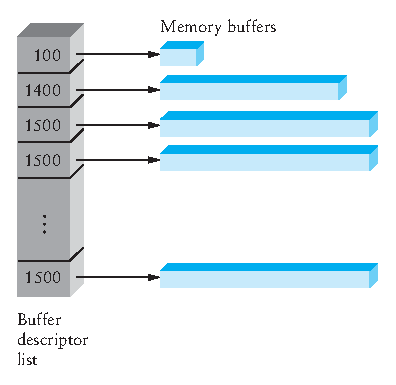
\includegraphics[height=2.1in]{figs/02x43}}
\itms{
  \item Idea: only use CPU to transfer control requests, not data
  \item Include list of buffer locations in main memory
  \ittms{
    \item Device reads list and accesses buffers through DMA
    \item Descriptions sometimes allow for scatter/gather I/O
  }
}
\end{slide}

\begin{slide}{Example: Network Interface Card}
\begin{centering}
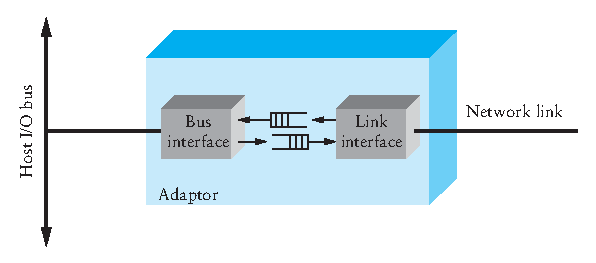
\includegraphics[height=1.5in]{figs/02x42} \\
\end{centering}
\itms{
  \item Link interface talks to wire/fiber/antenna
  \ittms{
    \item Typically does framing, link-layer CRC
  }
  \item FIFOs on card provide small amount of buffering
  \item Bus interface logic uses DMA to move packets to and from
    buffers in main memory
}
\end{slide}

\begin{slide}{Example: IDE disk read w.\ DMA}
\centerline{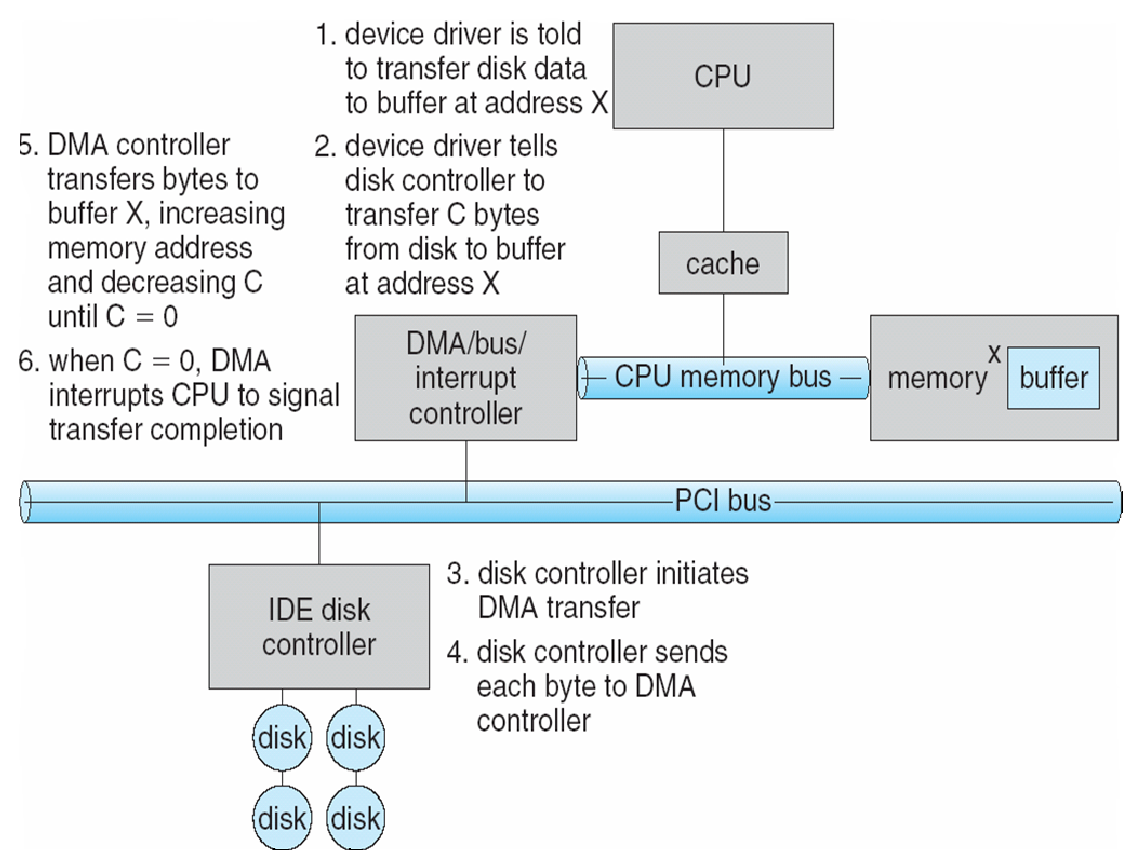
\includegraphics[height=70mm]{figs/dma}}
\end{slide}

\begin{slide}{Driver architecture}
\itms{
  \item Device driver provides several entry points to kernel
  \ittms{
    \item Reset, ioctl, output, interrupt, read, write, strategy \ldots
  }
  \item How should driver synchronize with card?
  \ittms{
    \item E.g., Need to know when transmit buffers free or packets arrive
    \item Need to know when disk request complete
  }
  \item One approach:  \emph{Polling}
  \ittms{
    \item Sent a packet?  Loop asking card when buffer is free
    \item Waiting to receive?  Keep asking card if it has packet
    \item Disk I/O?  Keep looping until disk ready bit set
  }
  \item Disadvantages of polling?
\pause
  \ittms{
    \item Can't use CPU for anything else while polling
    \item Or schedule poll in future and do something else, but then
	  high latency to receive packet or process disk block
  }
}
\end{slide}

\begin{slide}{Interrupt driven devices}
\itms{
  \item Instead, ask card to interrupt CPU on events
  \ittms{
    \item Interrupt handler runs at high priority
    \item Asks card what happened (xmit buffer free, new packet)
    \item This is what most general-purpose OSes do
  }
  \item Bad under high network packet arrival rate
  \ittms{
    \item Packets can arrive faster than OS can process them
    \item Interrupts are very expensive (context switch)
    \item Interrupt handlers have high priority
    \item In worst case, can spend 100\% of time in interrupt handler
	  and never make any progress -- \emph{receive livelock}
  \item Best:  Adaptive switching between interrupts
     and polling
  }
  \item Very good for disk requests
  \item Rest of today: Disks
}
\end{slide}

\section{Disk Drives}

\begin{slide}{Anatomy of a disk
    \cref{sched/readings/diskmodel.pdf}{[Ruemmler]}}
\itms{
\item Stack of magnetic platters
        \ittms{
        \item Rotate together on a central spindle @3,600-15,000 RPM
        \item Drive speed drifts slowly over time
        \item Can't predict rotational position after 100-200 revolutions
        }
\item Disk arm assembly
        \ittms{
        \item Arms rotate around pivot, all move together
        \item Pivot offers some resistance to linear shocks
        \item Arms contain disk heads--one for each recording surface
        \item Heads read and write data to platters
        }
}
\end{slide}

\begin{frame}
\frametitle{Disk}
\smallskip
\only<1>{\centerline{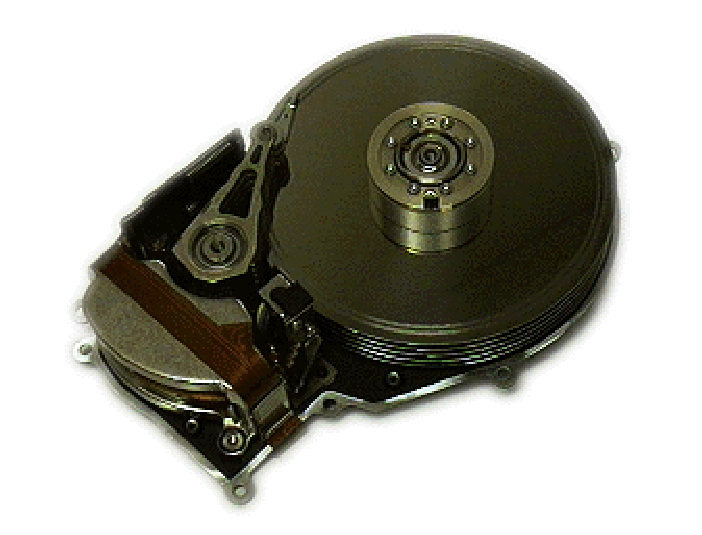
\includegraphics[height=2.8in]{figs/drive1.eps}}}
\only<2>{\centerline{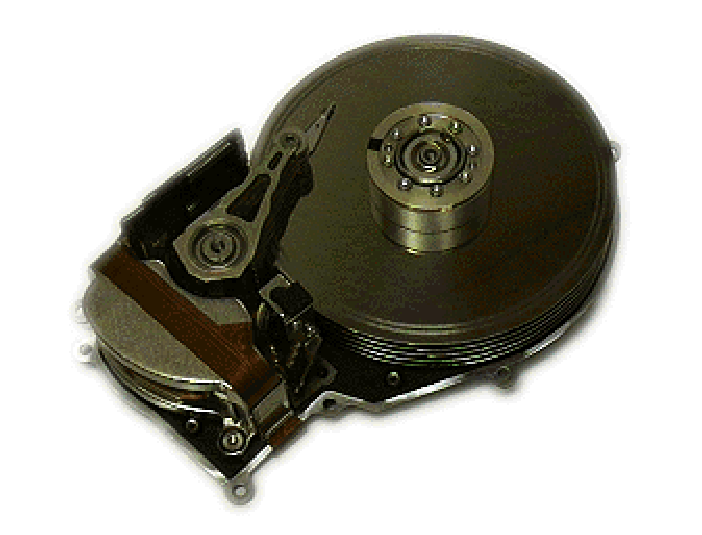
\includegraphics[height=2.8in]{figs/drive2.eps}}}
\only<3>{\centerline{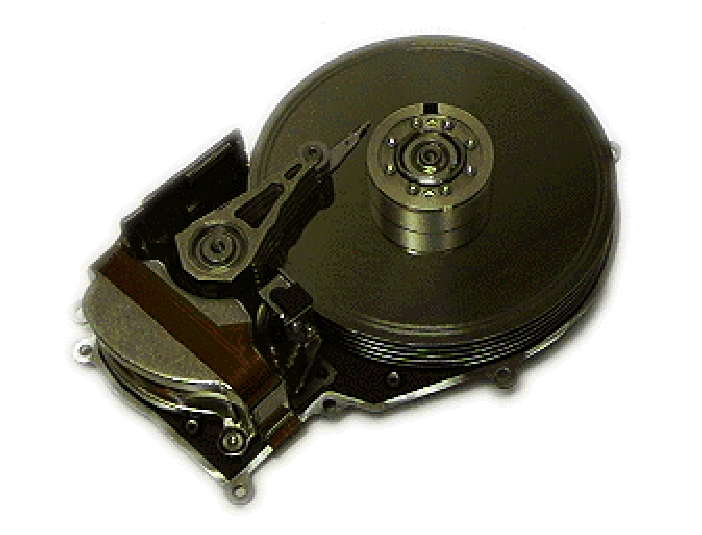
\includegraphics[height=2.8in]{figs/drive3.eps}}}
\end{frame}

\begin{slide}{Storage on a magnetic platter}
\itms{
\item Platters divided into concentric \emph{tracks}
\item A stack of tracks of fixed radius is a \emph{cylinder}
\item Heads record and sense data along cylinders
     \ittms{
     \item Significant fractions of encoded stream for error correction
     }
\item Generally only one head active at a time
     \ittms{
     \item Disks usually have one set of read-write circuitry
     \item Must worry about cross-talk between channels
     \item Hard to keep multiple heads exactly aligned
     }
}
\end{slide}

\begin{slide}{Cylinders, tracks, \& sectors}
\centerline{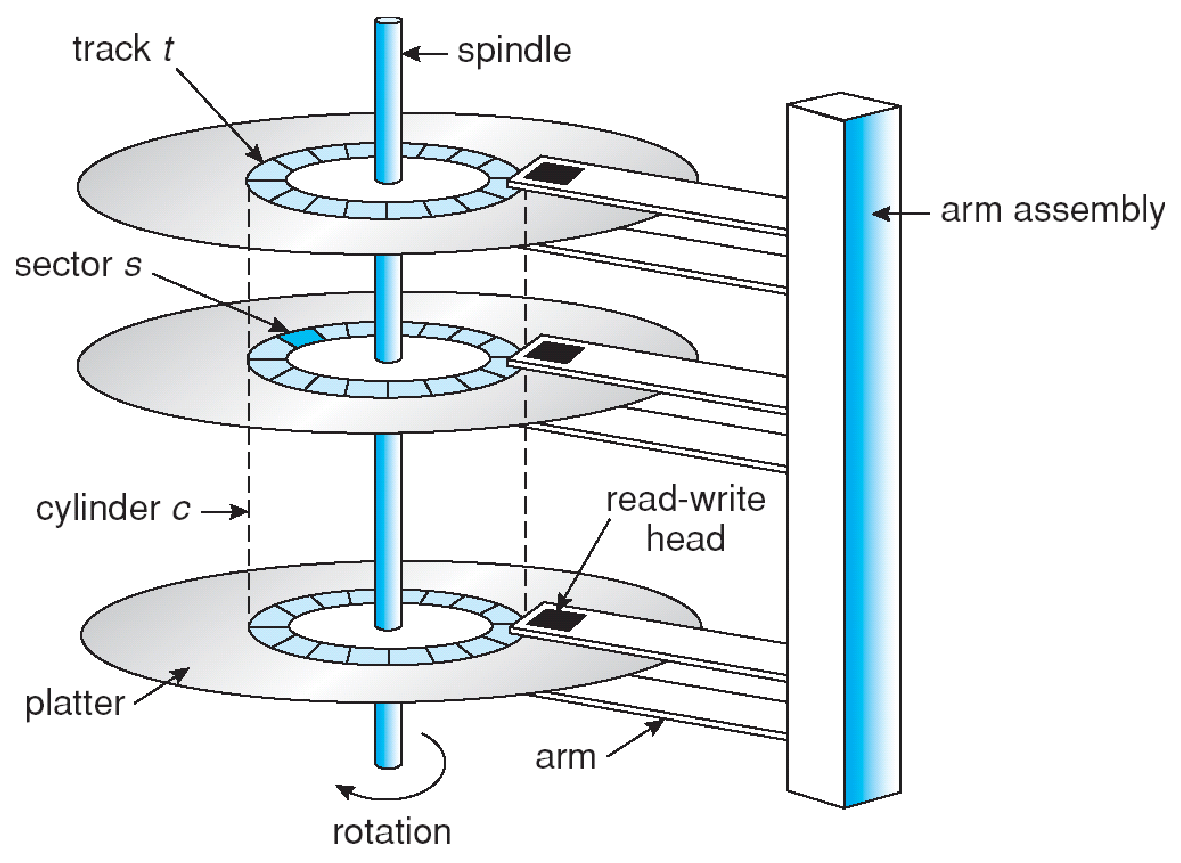
\includegraphics[height=2.8in]{figs/disk}}
\end{slide}

\begin{slide}{Disk positioning system}
\itms{
\item Move head to specific track and keep it there
        \ittms{
        \item Resist physical shocks, imperfect tracks, etc.
        }
\item A \textit{seek} consists of up to four phases:
  \ittms{
    \item\textit{speedup}--accelerate arm to max speed or half way point
    \item\textit{coast}--at max speed (for long seeks)
    \item\textit{slowdown}--stops arm near destination
    \item\textit{settle}--adjusts head to actual desired track
}
\item Very short seeks dominated by settle time ($\sim$1 ms)
\item Short (200-400 cyl.)\ seeks dominated by speedup
        \ittms{
        \item Accelerations of ~40g
        }
}
\end{slide}

\begin{slide}{Seek details}
\itms{
\item Head switches comparable to short seeks
        \ittms{
        \item May also require head adjustment
        \item Settles take longer for writes than for reads
          \only<1>{-- Why?}
\onslide<2->{
        \item[] If read strays from track, catch error with checksum,
          retry
        \item[] If write strays, you've just clobbered some other track
}
        }
\item Disk keeps table of pivot motor power
        \ittms{
        \item Maps seek distance to power and time
        \item Disk interpolates over entries in table
        \item Table set by periodic ``thermal recalibration''
        \item But, e.g., $\sim$500 ms recalibration every $\sim$25
              min bad for AV
        }
\item ``Average seek time'' quoted can be many things
        \ittms{
        \item Time to seek 1/3 disk, 1/3 time to seek whole disk
        }
}
\end{slide}

\begin{slide}{Transfer Time}
$Transfer~Time = Seek~Time + Rotational~Delay + MIN(Bus~Speed, Max~Read~Speed)$

\itms{
\gap
\item $Max~Read~Speed$ is determined by how fast we read sectors off the 
    platter:
\gap
}

$Max~Read~Speed = \frac{RPM}{60 sec/min} \times Bytes~per~Sector \times 
    Sectors~per~Track$

\itms{
\gap
\item $Rotational~Delay$ is how long it takes on average to rotate the platter 
    into position (i.e.~half a rotation of the platter).
\gap
}

$Rotational~Delay = \frac{1}{2} \times \frac{60 sec/min}{RPM}$

\end{slide}

\begin{frame}<1-2>
\frametitle{Sectors}
\itms{
\item Disk interface presents linear array of \emph{sectors}
	\ittms{
	\item Generally 512 bytes, written atomically (even if power
          failure)
	}
\item Disk maps logical sector \#s to physical sectors
	\ittms{
	  \item \textit{Zoning}--puts more sectors on longer tracks
	  \item \textit{Track skewing}--sector 0 pos.\ varies by track
	  \alt<1>{(why?)}{\rlap{(sequential access speed)}}
	  \item \textit{Sparing}--flawed sectors remapped elsewhere
	 }
\item OS doesn't know logical to physical sector mapping
	\ittms{
	\item Larger logical sector \# difference means larger seek
	\item Highly non-linear relationship (\textit{and} depends on zone)
	\item OS has no info on rotational positions
	\item Can empirically build table to estimate times
	}
}
\end{frame}

\begin{slide}{Disk interface}
\itms{
\item Controls hardware, mediates access
\item Computer, disk often connected by bus (e.g., SCSI)
	\ittms{
	\item Multiple devices may contentd for bus
}
\item \Red{Possible disk/interface features:}
\item Disconnect from bus during requests %(+200 $\mu$s SCSI)
\item Command queuing:  Give disk multiple requests
	\ittms{
	\item Disk can schedule them using rotational information
	}
\item Disk cache used for read-ahead
	\ittms{
	\item Otherwise, sequential reads would incur whole revolution
	\item Cross track boundaries?  Can't stop a head-switch
	}
\item Some disks support write caching
	\ittms{
	\item But data not stable---not suitable for all requests
	}
}
\end{slide}

\iffalse

\section{SCSI}

\begin{slide}{SCSI overview \cref{sched/readings/scsi.pdf}{[Schmidt]}}
\itms{
  \item SCSI \emph{domain} consists of devices and an SDS
  \ittms{
    \item Devices:  host adapters \& SCSI controllers
    \item \emph{Service Delivery Subsystem} connects devices---e.g., SCSI bus
  }
  \item SCSI-2 bus (SDS) connects up to 8 devices
  \ittms{
    \item Controllers can have $>1$ ``logical units'' (LUNs)
    \item Typically, controller built into disk and 1 LUN/target, but
          ``bridge controllers'' can manage multiple physical devices
  }
  \item Each device can assume role of \emph{initiator} or \emph{target}
  \ittms{
    \item Traditionally, host adapter was initiator, controller target
    \item Now controllers act as initiators (e.g., \textsc{copy} command)
    \item Typical domain has $1$~initiator, $\ge1$ targets
  }
}
\end{slide}

\begin{slide}{SCSI requests}
\itms{
  \item A \emph{request} is a command from initiator to target
  \ittms{
    \item Once transmitted, target has control of bus
    \item Target may disconnect from bus and later reconnect \\
       (very important for multiple targets or even multitasking)
  }
  \item Commands contain the following:
  \ittms{
    \item \emph{Task identifier}---initiator ID, target ID, LUN, tag
    \item \emph{Command descriptor block}---e.g., read 10 blocks
	    at pos.\ $N$
    \item Optional \emph{task attribute}---\textsc{simple},
      \textsc{ordered}, \textsc{head of queue}
    \item Optional:  output/input buffer, sense data
    \item \emph{Status byte}---\textsc{good, check condition,
  intermediate}, $\ldots$
  }
}
\end{slide}

\begin{slide}{Executing SCSI commands}
\itms{
  \item Each LUN maintains a queue of \emph{tasks}
  \ittms{
    \item Each task is \textsc{dormant}, \textsc{blocked},
      \textsc{enabled}, or \textsc{ended}
    \item \textsc{simple} tasks are dormant until no ordered/head of queue
    \item \textsc{ordered} tasks dormant until no HoQ/more recent ordered
    \item \textsc{HoQ} tasks begin in enabled state
  }
  \item Task management commands available to initiator
  \ittms{
    \item Abort/terminate task, Reset target, etc.
  }
  \item Linked commands
  \ittms{
    \item Initiator can link commands, so no intervening tasks
    \item E.g., could use to implement atomic read-modify-write
    \item Intermediate commands return status byte \textsc{intermediate}
  }
}
\end{slide}

\begin{slide}{SCSI exceptions and errors}
\itms{
  \item After error stop executing most SCSI commands
  \ittms{
    \item Target returns with \textsc{check condition} status
    \item Initiator will eventually notice error
    \item Must read specifics w.\ \textsc{request sense}
  }
  \item Prevents unwanted commands from executing
  \ittms{
    \item E.g., initiator may not want to execute 2nd write if 1st fails
  }
  \item Simplifies device implementation
  \ittms{
    \item Don't need to remember more than one error condition
  }
  \item Same mechanism used to notify of media changes
  \ittms{
    \item I.e., ejected tape, changed CD-ROM
  }
}
\end{slide}

\fi

\begin{slide}{Disk performance}
\itms{
  \item Placement \& ordering of requests a huge issue
  \ittms{
    \item Sequential I/O much, much faster than random
    \item Long seeks much slower than short ones
    \item Power might fail any time, leaving inconsistent state
  }
  \item Must be careful about order for crashes
  \ittms{
    \item More on this in next two lectures
  }
  \item Try to achieve contiguous accesses where possible
  \ittms{
    \item E.g., make big chunks of individual files contiguous
  }
  \item Try to order requests to minimize seek times
  \ittms{
    \item OS can only do this if it has a multiple requests to order
    \item Requires disk I/O concurrency
    \item High-performance apps try to maximize I/O concurrency
  }
  \item Next:  How to schedule concurrent requests
}
\end{slide}

\iffalse

\section{Disk Scheduling}

\begin{slide}{Scheduling: FCFS}
\itms{
\item ``First Come First Served''
\ittms{
        \item Process disk requests in the order they are received
}
\item Advantages
	\ittms{
\onslide<2->{
	\item Easy to implement
	\item Good fairness
	}
}
\item Disadvantages
	\ittms{
\onslide<2>{
	\item Cannot exploit request locality
	\item Increases average latency, decreasing throughput
	}
}
}
\end{slide}

\begin{slide}{FCFS example}
\centerline{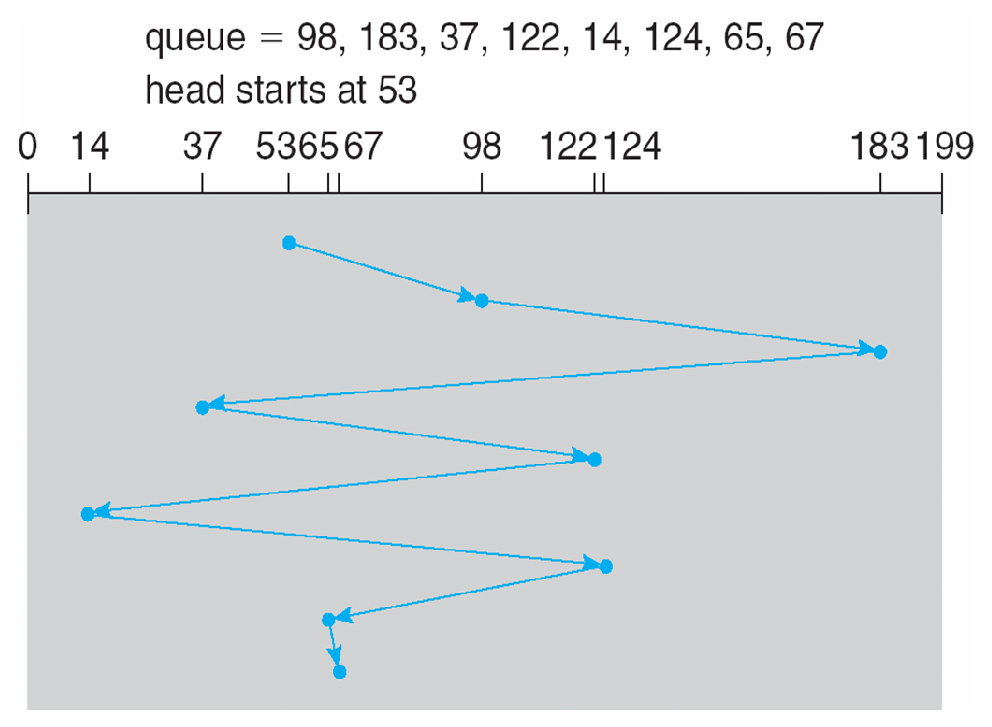
\includegraphics[width=4in]{figs/fcfs}}
\end{slide}

\begin{slide}{Shortest positioning time first (SPTF)}
\itms{
\item Shortest positioning time first (SPTF)
\ittms{
        \item Always pick request with shortest seek time\color[rgb]{1,1,1}
}
\item Also called Shortest Seek Time First (SSTF)
\item Advantages
	\ittms{
\onslide<2->{
	\item Exploits locality of disk requests
	\item Higher throughput
	}
}
\item Disadvantages
	\ittms{
\onslide<2->{
	\item Starvation
	\item Don't always know what request will be fastest
	}
}
\onslide<2->
\item Improvement\alt<3->{:  Aged SPTF}{?}
  \onslide<3->{
	\ittms{
	\item Give older requests higher priority
	\item Adjust ``effective'' seek time with weighting factor: \\
	\(T_{\mathrm{eff}} = T_{\mathrm{pos}} - W\cdot T_{\mathrm{wait}}\)
	}
}
}
\end{slide}

\begin{slide}{SPTF example}
\centerline{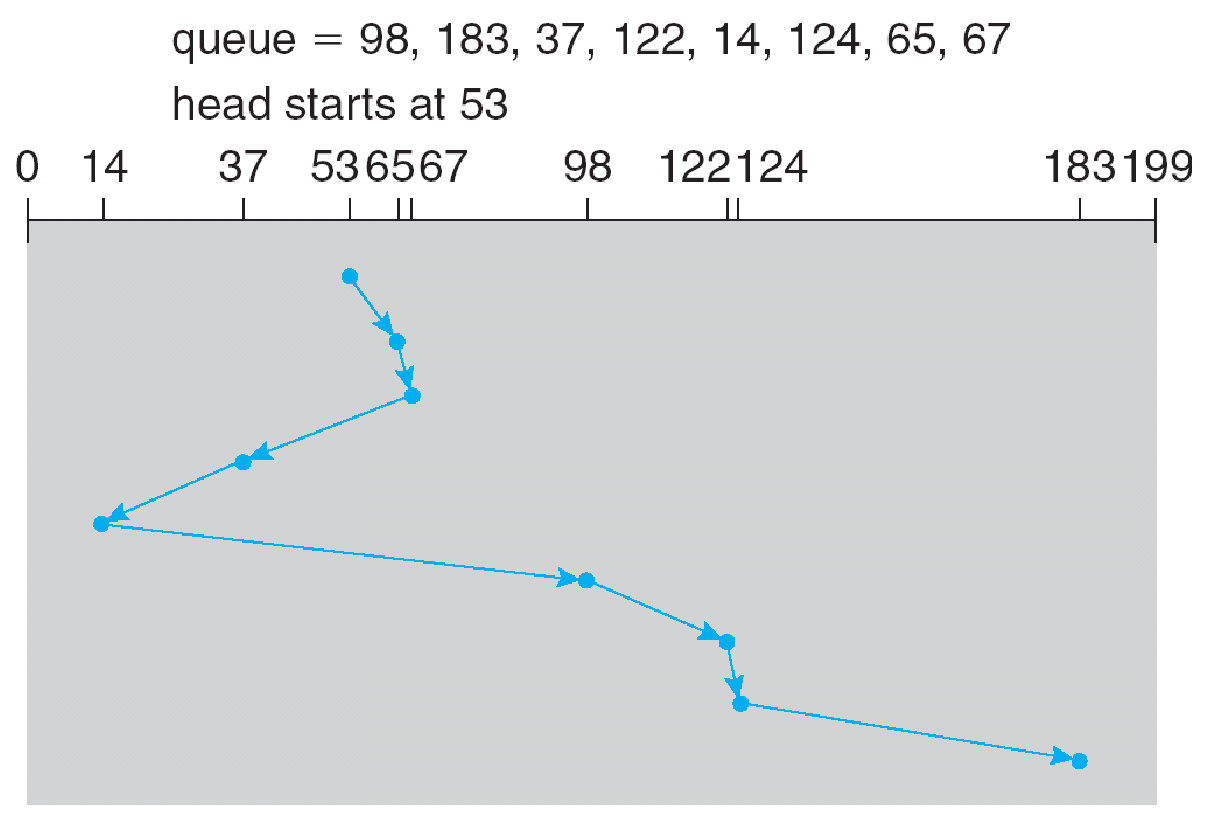
\includegraphics[width=4in]{figs/sptf}}
\end{slide}

\begin{slide}{``Elevator'' scheduling (SCAN)}
\itms{
\item Sweep across disk, servicing all requests passed
	\ittms{
	\item Like SPTF, but next seek must be in same direction
	\item Switch directions only if no further requests
	}
\item Advantages
	\ittms{
\onslide<2->{
	\item Takes advantage of locality
	\item Bounded waiting
	}
        }
\item Disadvantages
	\ittms{
\onslide<2->{
	\item Cylinders in the middle get better service
	\item Might miss locality SPTF could exploit
	}
        }
\onslide<2->
\item CSCAN:  Only sweep in one direction\\
	\Red{Very commonly used algorithm in Unix}
\item Also called LOOK/CLOOK in textbook
\ittms{
  \item (Textbook uses [C]SCAN to mean scan entire disk uselessly)
}
}
\end{slide}

\begin{slide}{CSCAN example}
\centerline{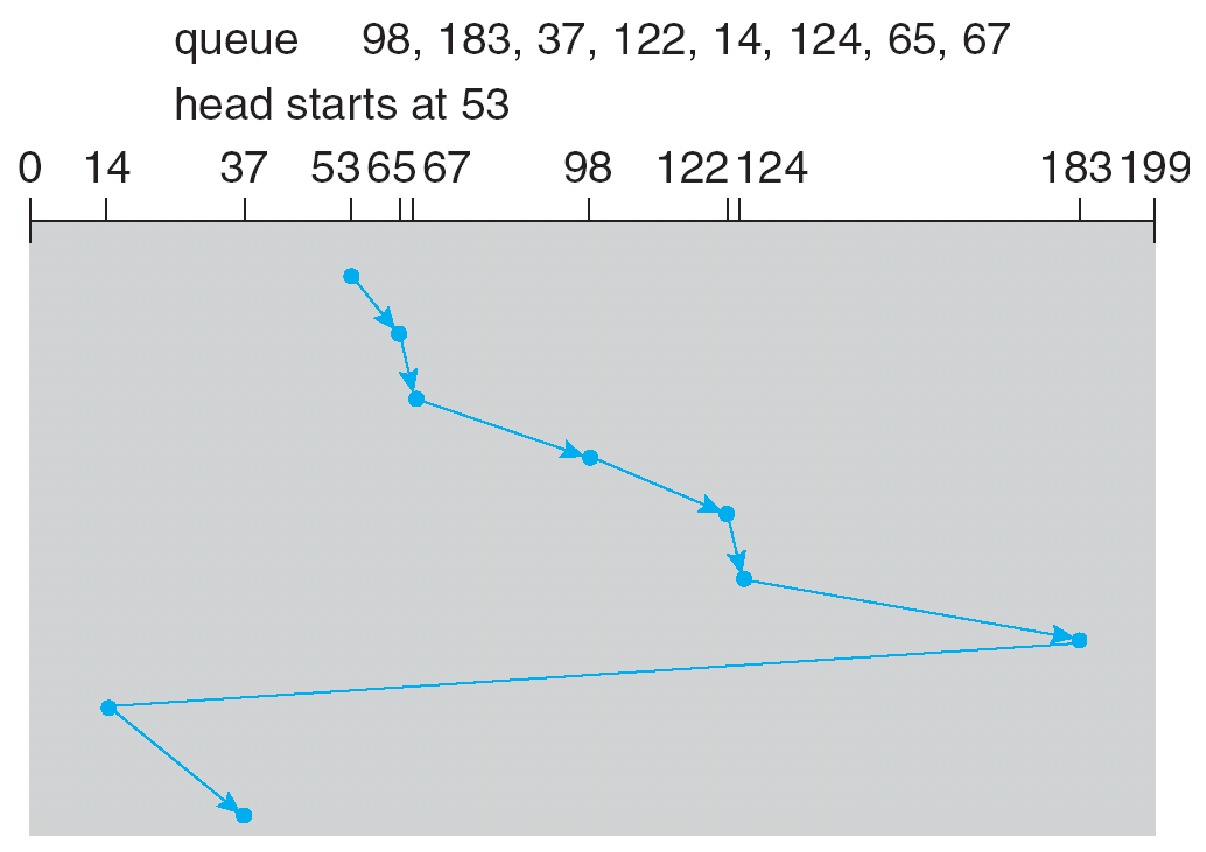
\includegraphics[width=4in]{figs/clook}}
\end{slide}

\begin{slide}{VSCAN(r)}
\itms{
\item Continuum between SPTF and SCAN
	\ittms{
	\item Like SPTF, but slightly changes ``effective'' positioning
	  time \\
If request in same direction as previous seek:
  \(T_{\mathrm{eff}} = T_{\mathrm{pos}}\)\\
Otherwise:
  \(T_{\mathrm{eff}} = T_{\mathrm{pos}} + r\cdot T_{\mathrm{max}}\)
	\item when r = 0, get SPTF, when r = 1, get SCAN
	\item E.g., r = 0.2 works well
	}
\item Advantages and disadvantages
	\ittms{
	\item Those of SPTF and SCAN, depending on how r is set
	}

   \item See
     \href{http://www.ece.cmu.edu/~ganger/papers/sigmetrics94.pdf}%
          {[Worthington]} for good description and evaluation of
          various disk scheduling algorithms
}
\end{slide}

\fi

\section{Flash Storage}

\begin{slide}{Flash memory}
\itms{
  \item Today, people increasingly using flash memory
  \item Completely solid state (no moving parts)
  \ittms{
    \item Remembers data by storing charge
    \item Lower power consumption and heat
    \item No mechanical seek times to worry about
  }
  \item Limited \# overwrites possible
  \ittms{
    \item Blocks wear out after 10,000 (MLC) -- 100,000 (SLC) erases
    \item Requires \emph{flash translation layer} (FTL) to provide
      \emph{wear leveling}, so repeated writes to logical block
      don't wear out physical block
    \item FTL can seriously impact performance
    \item In particular, random writes \emph{very} expensive
\href{http://research.microsoft.com/pubs/63681/TR-2005-176.pdf}{[Birrell]}
  }
  \item Limited durability
  \ittms{
    \item Charge wears out over time
    \item Turn off device for a year, you can easily lose data
  }
}
\end{slide}

\begin{slide}{Types of flash memory}
\itms{
  \item NAND flash (most prevalent for storage)
  \ittms{
    \item Higher density (most used for storage)
    \item Faster erase and write
    \item More errors internally, so need error correction
  }
  \item NOR flash
  \ittms{
    \item Faster reads in smaller data units
    \item Can execute code straight out of NOR flash
    \item Significantly slower erases
  }
  \item Single-level cell (SLC) vs.\ Multi-level cell (MLC)
  \ittms{
    \item MLC encodes multiple bits in voltage level
    \item MLC slower to write than SLC
  }
}
\end{slide}

\begin{slide}{NAND Flash Overview}
\itms{
  \item Flash device has 2112-byte \emph{pages}
  \ittms{
    \item 2048 bytes of data + 64 bytes metadata \& ECC
  }
  \item \emph{Blocks} contain 64 (SLC) or 128 (MLC) pages
  \item Blocks divided into 2--4 \emph{planes}
  \ittms{
    \item All planes contend for same package pins
    \item But can access their blocks in parallel to overlap latencies
  }
  \item Can \emph{read} one page at a time
  \ittms{
    \item Takes 25 $\mu\mathrm s$ + time to get data off chip
  }
  \item Must \emph{erase} whole block before \emph{programming}
  \ittms{
    \item Erase sets all bits to 1---very expensive (2 msec)
    \item Programming pre-erased block requires moving data to
      internal buffer, then 200 (SLC)--800 (MLC)~$\mu\mathrm s$
  }
}
\end{slide}

\begin{slide}{Flash Characteristics
    \href{http://cseweb.ucsd.edu/~swanson/papers/Asplos2009Gordon.pdf}{[Caulfield'09]}}
\centerline{
\begin{tabular}{|r|c|c|}
\hline
\textbf{Parameter}\hfill & \textbf{SLC} & \textbf{MLC} \\\hline
%\multicolumn{3}{|l|}{\textbf{Chip Configuration}}\\\hline
Density Per Die (GB) & 4 & 8 \\
Page Size (Bytes) & 2048+32 & 2048+64 \\
Block Size (Pages) & 64 & 128 \\
%Bus Width (Bits) & 16 & 16 \\
\hline
%\multicolumn{3}{|l|}{\textbf{Operational Latencies ($\mu \mathrm s$)}}\\\hline
Read Latency ($\mu\mathrm s$) & 25 & 25 \\
Write Latency ($\mu\mathrm s$) & 200 & 800 \\
Erase Latency ($\mu\mathrm s$) & 2000 & 2000 \\
\hline
 40MHz, 16-bit bus \hfill   Read b/w (MB/s)& 75.8  &  75.8 \\
           Program b/w (MB/s)& 20.1  &  5.0 \\
133MHz \hfill   Read b/w (MB/s)& 126.4 & 126.4 \\
           Program b/w (MB/s)& 20.1  &  5.0 \\
%400MHz (projected) \hfill   Read b/w (MB/s)& 161.1 & 161.1 \\
           %Program b/w (MB/s)& 20.1  &  5.0 \\
\hline
\end{tabular}}
\end{slide}

% http://www.t13.org/documents/UploadedDocuments/project/d1410r3b-ATA-ATAPI-6.pdf

\end{document}
